\chapter{Ancillary calculations}\label{apx:ancillary-calculations}


\section{Evolution under a gravitational Hamiltonian}\label{apx:general-state-gravitaional-hamiltonian}
In this section the time evolution of a system under Hamiltonian eq. \eqref{eq:2:gravity-hamiltonian} is calculated for two particles $A$ and $B$ (mass $m$) separated by $L$ in a harmonic trap (frequency $\omega$). A example from Ref. \cite{Carney_2018} is followed.
The total Hamiltonian describing the dynamics is given by
\begin{equation}
  \op{H} = \sum_{i=A,B} \frac{\op{p}_i}{2m} + \frac{1}{2} m \omega^2 \op{x}_i^2 + \op{H}_G
\end{equation}
where $\op{x}$ and $\op{p}$ are the position and momentum operators of the particle satisfying the canonical commutator relation $[\op{x}_i, \op{p}_j] = i \hbar \delta_{ij}$.
Introducing ladder operators $\op{x}_i = \sqrt{\hbar/2m\omega} \left(\op{a_i}^\dagger + \op{a_i}\right)$, $\op{p}_i = \sqrt{\hbar m \omega /2} \left(\op{a_i}^\dagger - \op{a_i}\right)$, the Hamiltonian can be rewritten:
\begin{equation}
  \op{H} = \sum_{i=A,B} \hbar \omega \op{a}_i^\dagger\op{a}_i - \frac{Gm^2}{L^3}\left(\sqrt{\frac{\hbar}{2m\omega}}\right)^2 \left(\op{a}_A\op{a}_B + \op{a}_A\op{a}^\dagger_B + \op{a}^\dagger_A\op{a}_B + \op{a}^\dagger_A\op{a}^\dagger_B\right) .
\end{equation}
Applying the rotating wave approximation, the term $\op{a}_A\op{a}_B + \op{a}^\dagger_A\op{a}^\dagger_B$ can be dropped. The effective Hamiltonian is therefore in the form
\begin{equation}
  \op{H}_\mathrm{eff} = \sum_{i=A,B} \hbar \omega \op{a}_i^\dagger\op{a}_i - \hbar g \left(\op{a}_A\op{a}^\dagger_B + \op{a}^\dagger_A\op{a}_B\right)
\end{equation}
with coupling strength $g=Gm/\omega L^3$.
A general biparty Fock state $\ket{\psi_0} = \ket{kl}$ with $k, l \in \mathbb{N}_0$ can be evolved in time under this hamiltonian, treating the gravitational interaction $H_G = -\hbar g (\op{a}_1\op{a}_2^\dagger + \op{a}_1^\dagger\op{a}_2)$ as a perturbation. 
The resulting state $\ket{\psi(t)}$ after some time $t$ is in the most general form given as
\begin{equation}
  \ket{\psi(t)} = \sum_{i, j \geq 0} c_{i,j}(t) \ket{i,j}
\end{equation}
where the coefficients $c_{i,j}(t)$ are given by first order perturbation theory as
\begin{equation}
  c_{i,j}(t) = c_{i,j}(t = 0) - \frac{i}{\hbar} \int_0^t \dd t' \bra{ij}\op{H}_G\ket{kl} e^{-i(E_{kl}-E_{ij})t'/\hbar} .
\end{equation}
The exponent is given by the energy of the appropriate Fock states $E_{kl}-E_{ij} = \hbar \omega (k+l - (i+j))$ and the matrix element in the integrand can be calculated to
\begin{equation}
  \bra{ij}\op{H}_G\ket{kl} =
  \begin{cases}
    -\hbar g & \text{if } i = k \pm 1 \text{ and } j = l \mp 1 \\
    0 & \text{otherwise}
  \end{cases}.
\end{equation}
The coefficients for $t=0$ are trivially given from the initial state as
\begin{equation}
  c_{i,j}(t=0) = \begin{cases}
    1 & \text{for } i,j = k,l \\
    0 & \text{otherwise}
  \end{cases}.
\end{equation}
For the non-zero states the energies in the exponent equate to zero and the evolved state is given by (up to a normalization)
\begin{equation}\label{eq:apx:perturbation-result}
  \ket{\psi(t)} = \ket{kl} - i g t \ket{k-1,l+1} - i g t \ket{k+1,l-1} + \mathcal{O}(g^2).
\end{equation}
For $k=1$ and $l=0$, the evolved state is in the form (with normalization $\mathcal{N}$)
\begin{equation}
  \ket{\psi(t)} = \mathcal{N} \left(\ket{10} - igt\ket{01 + \mathcal{O}(g^2)}\right)
\end{equation}
which is entangled with logarithmic negativity $E_N(\ketbra{\psi(t)}) \simeq 2tg/\log 2 + \mathcal{O}(g^2) \geq 0$.



\section{Exemplary calculation of the logarithmic negativity}\label{apx:E_N-exemplary}
In this section, the logarithmic negativity $E_N$ eq. \eqref{eq:2:logarithmic-negativity} is exemplary calculated for the state eq. \eqref{eq:2:evolved-state}.
The density matrix of this system is given by
\begin{equation}
  \rho(t) = \ketbra{\psi(t)} = \frac{1}{4}
  \begin{pmatrix}
    1 & e^{i\Delta\phi}  & e^{i\Delta\phi} & 1 \\
    e^{-i\Delta\phi} & 1 & 1  & e^{-i\Delta\phi} \\
    e^{-i\Delta\phi} & 1  & 1 & e^{-i\Delta\phi} \\
    1 & e^{i\Delta\phi} & e^{i\Delta\phi} & 1
  \end{pmatrix}.
\end{equation}
Consequently, the partially transposed density $\rho^{\Gamma_B}$ is given by
\begin{equation}
  \rho^{\Gamma_B}(t) = \frac{1}{4}
  \begin{pmatrix}
    1 & e^{-i\Delta\phi}  & e^{i\Delta\phi} & 1 \\
    e^{i\Delta\phi} & 1 & 1  & e^{-i\Delta\phi} \\
    e^{-i\Delta\phi} & 1  & 1 & e^{i\Delta\phi} \\
    1 & e^{i\Delta\phi} & e^{-i\Delta\phi} & 1
  \end{pmatrix}.
\end{equation}
The eigenvalues where calculated using \texttt{Mathematica} and equate to
\begin{equation*}
  \left\{ \sin^2\left(\frac{\Delta\phi}{2}\right), \cos^2\left(\frac{\Delta\phi}{2}\right), \frac{\sin\Delta\phi}{2}, -\frac{\sin\Delta\phi}{2} \right\}
\end{equation*}
According to \cref{lemma:trace-norm-hermitian}, $\norm{\rho^{\Gamma_B}}_1$ is given by the sum of the absolute eigenvalues, which is equal to $1+\abs{\sin\Delta\phi}$. The negativity as the absolute sum of all negative eigenvalues (demonstrated in \cref{proposition:negativity}) equates to $\mathcal{N} = \abs{\sin\Delta\phi}/2$. Both methods result in a logarithmic negativity of $E_N = \log_2(1 + \abs{\sin\Delta\phi})$.




\section{Polarizability of a dielectric sphere}
\label{apx:polarizability-sphere}

The polarizability $\alpha$ is defined via
\begin{equation}
  \vec{E_\infty} \alpha = \vec{p},
\end{equation}
where $\vec{p}$ is the induced dipole moment and $\vec{E_\infty}$ is the external electric field that induces the dipole moment. For a linear and uniform dielectric, it is given as $\vec{p} = \mathcal{V} \varepsilon_0 (\varepsilon_r - 1) \vec{E_\mathrm{in}}$ \cite[p. 220-226]{Griffiths_2018}. Here, $\mathcal{V}$ is the volume of the object and $\vec{E_\mathrm{in}}$ is the electric field inside the dielectric.
The electrostatic boundary conditions for the problem are given by
\begin{equation}
  V_\mathrm{in} \big|_{r=R} = V_\mathrm{out} \big|_{r=R} 
  \quad \text{and} \quad 
  \varepsilon_r\varepsilon_0\pdv{V_\mathrm{in}}{r}\bigg|_{r=R} = \varepsilon_0\pdv{V_\mathrm{out}}{r} \bigg|_{r=R}
\end{equation}
and the electric potential outside of the sphere at $r\rightarrow\infty$ should be equal to the external dipole-inducing field $V_\mathrm{out} |_{r\rightarrow\infty} = -\vec{E_\infty} \cdot \vec{r} = -E_\infty r\cos\theta$.
The electric potential inside and outside the sphere can be calculated using the spherical decomposition of the general electric potential $V \propto 1/\abs{\vec{r} - \vec{r'}}$ into Legendre Polynomials $P_l$ \cite[p. 188-190]{Griffiths_2018}:
\begin{align}
  V_\mathrm{in}(r, \theta) &= -E_\infty r\cos\theta + \sum_{l=0}^{\infty} A_l r^l P_l(\cos\theta), \\
  V_\mathrm{out}(r, \theta) &= -E_\infty r \cos\theta + \sum_{l=0}^{\infty} \frac{B_l}{r^{l+1}} P_l(\cos\theta).
\end{align}
Applying both boundary conditions, it follows that \cite[p. 249-251]{Griffiths_2018}
\begin{equation}
  \begin{cases}
    A_l = B_l = 0 & \text{for } l \neq 1, \\
  A_1 = -\frac{3}{\varepsilon_r + 2}E_\infty, \quad B_1 = \frac{\varepsilon_r-1}{\varepsilon_r + 2}R^3E_\infty
  \end{cases}
\end{equation}
and the resulting  homogenous electric field $\vec{E_\mathrm{in}} = -\vec{\nabla} V_\mathrm{in}$ inside the sphere is given as
\begin{equation}
  \vec{E_\mathrm{in}} = \frac{3}{\varepsilon_r + 2} \vec{E_\infty} .
\end{equation}
The field is shown on the right in \cref{fig:apx:dielectric-sphere-field}.The polarizability $\alpha$ of the sphere can be now be determined to
\begin{equation}
  \alpha_\mathrm{sphere} = 4\pi \varepsilon_0 R^3 \left(\frac{\varepsilon_r - 1}{\varepsilon_r + 2}\right).
\end{equation}
Depending on the definition, sometimes the factor $4\pi\varepsilon_r$ is dropped.
\begin{figure}[!htbp]
  \centering
  \begin{subfigure}[b]{0.48\textwidth}
      \centering
      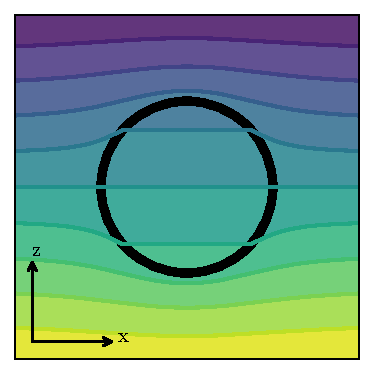
\includegraphics[width=\textwidth]{./../figures/potential-dielectric-sphere-small.pdf}
  \end{subfigure}
  \hfill
  \begin{subfigure}[b]{0.48\textwidth}
      \centering
      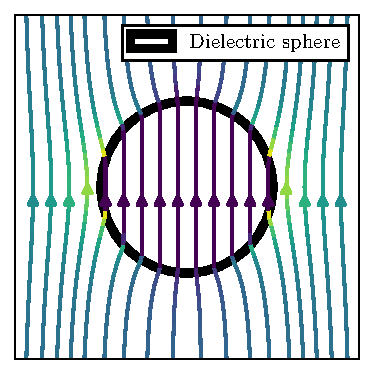
\includegraphics[width=\textwidth]{./../figures/others/field-dielectric-sphere-small.pdf}
  \end{subfigure}
  \caption{\textbf{left:} Electric potential $V$ of a dielectric sphere in a external electric field $\vec{E_\infty} \parallel \vec{e_z}$. \textbf{right:} The corresponding electric field lines inside and outside the dielectric sphere.}
  \label{fig:apx:dielectric-sphere-field}
\end{figure}




\section{Blocking of the shield}\label{apx:blocking-of-the-shield}
Assume two spheres $A$ and $B$ with charge $q_A$ and $q_B$ separated by a distance $2L$ on the $x$-axis. A circular shield is placed perfectly in the center of the spheres orthogonal to the direct connection between them. The magnitude of the field at a distance $z$ in the direction $\vec{e}_x$ from this connection line is given by 
\begin{equation}
  E_x(z) = \frac{L(q_A - q_B)}{4\pi\varepsilon_0 (L^2 + z^2)^{3/2}}
\end{equation}
The total flux through the circular shield with radius $r_s$ is given by
\begin{equation}
  \Phi = \int_{0}^{r_s}\dd z \int_{0}^{2\pi} z \dd \varphi \, E_x(z) = \frac{(q_A - q_B)}{2 \varepsilon_0} \left[ 1 - \frac{L}{\sqrt{L^2 + r_s^2}} \right] .
\end{equation}
Comparing the total flux for $r_s \rightarrow \infty$ with the flux through the shield, one can arrive at the charge-independent \emph{effectiveness} $\eta$ of the shield as
\begin{equation}
  \eta = \frac{\Phi}{\Phi_\infty} = 1 - \frac{L}{\sqrt{L^2 + r_s^2}}
\end{equation}
and thus a shield with radius
\begin{equation}
  r_s = L \sqrt{\frac{1 - (1-\eta)^2}{(1-\eta)^2}}
\end{equation}
will block a fraction $\eta$ of the total field.




\section{Thermal harmonic oscillator}\label{apx:thermal-harmonic-oscillator}
The amplitude $z$ of a single vibrational shield-mode $(k,l)$ with frequency $\omega_{kl} \equiv \omega$ behaves like a quantum harmonic oscillator. 
The average amplitude $\avg{z}_n = 0$. 
The variance $(\Delta z)^2 = \avg{z^2} - \avg{z}^2$ however is given by
\begin{equation}
  (\Delta z)^2_n = \avg{z^2}_n = \frac{\hbar}{2m\omega} (1+2n) .
\end{equation}
At a temperature $T$, the occupation of the modes is described by the boltzmann distribution:
\begin{equation}\label{eq:apx:thermal-oscillator-variance}
  \avg{z^2}_T = \sum_{n=0}^{\infty} \frac{1}{Z} e^{-\beta E_n} \avg{z^2}_n,
\end{equation}
where $\beta = 1/k_B T$, $E_n = \hbar \omega (n+1/2)$ is the energy of mode $n$ and
\begin{equation}
  Z = \sum_{n=0}^{\infty} e^{-\beta E_n} = \frac{e^{-\beta \frac{\hbar \omega}{2}}}{1-e^{-\beta \hbar \omega}}
\end{equation}
is the partition function. Using known series, the expression eq. \eqref{eq:apx:thermal-oscillator-variance} can be evaluated to
\begin{align}
  (\Delta z)^2_T = \avg{z^2}_T &= \frac{\hbar}{2m\omega} \sum_{n=0}^{\infty} \frac{1}{Z}\left[e^{-\beta E_n} + 2ne^{-\beta E_n}\right] \\
  &= \frac{\hbar}{2m\omega} \left[1 + \frac{2}{Z}\sum_{n=0}^{\infty} n e^{-\beta E_n}\right] \\
  &= \frac{\hbar}{2m\omega} \left[1 + \frac{2e^{-\beta\hbar\omega}}{1-e^{-\beta\hbar\omega}} \right] = \frac{\hbar}{2m\omega} \coth(\frac{\hbar \omega}{2 k_B T})
\end{align}